
\chapter{Search by Face Similarity}

% Research in past several decades proved that human have extreme capability of recognizing the faces. Faces are so special to us as a species, that we are able to ..... We are able to recall that we met specific person dating the meeting years back. Therefore we state a question, if the search based only on faces can be done.

% This approach organizes the space of seen faces to help the user to orientate and find the search face. Though, in order to describe the face space we use deep encodings trained by a network used for face recognition.

% In the previous chapter we elaborated an approach to search in dataset using objects and their spatial information. In this chapter we investigate a different option -- traversion using faces. The question we ask is if it is possible to find a specific scene by showing user faces. Since there is a limitation of how many faces we can display at once to the user, we will investigate if we can lead user to the specific scene with specific face via traversion through multiple similar faces.

% Since the similarity of faces is a strongly abstract perception we rely on feature representation of the faces. This helps us to create an interactive environment to traverse via huge aount of faces and test our hypothesis, if this approach can be used for scene searching. 

% This chapter firstly introduces different approaches to obtaining face representations. Then we proceed by presenting different approaches for traversion over dataset of faces. At the end of the chapter we present the results in our specific task -- scene search .

% \todo[inline]{ motivation - otestovat hypotezu ci je to mozne a nejaky nahlad ako ot moze vyzerat}
% \section{Preliminaries}
% \todo[inline]{face features - popisat zdroj siete}
% \section{Creating SOM Representation of the face space}
% \section{Evaluation}

Content-based image retrieval approaches the problem of finding images relevant from an image database based on visual features. These visual features are nowadays extracted through a wide range of automatic extraction methods. As the research of deep neural networks advanced, an ability of the networks to cover not only low-level visual features but also high-level semantic concepts unveiled. Despite these uncoverings, the high-level features may not correspond to the common features viewed by a human. This gap is also often enhanced by the high dimensionality of the features and because of that a hidden structure in these features. Since these features often lack one to one correspondence with humanly perceived features, it leads to difficulties in the task of exploration.

In this chapter, we aim to research an approach of using visual features obtained by a neural network for a human face. Due to the fact, that these features often do not have one to one correspondence with human perception (i.e. human may notice the color of the eyes, the network may not have a specific feature for it, rather a combination of multiple features, or not at all), we shift from single-round query to navigational queries, where a single retrieval instance consists of multiple rounds of user-system interaction.

Our task is to verify the option, to search the dataset of the images based only on the people in the images using deep features for their faces. To provide an ability to search through a high-dimensional space of faces we incorporate navigational ability through the dataset.

The goal is to yet again to find a particular scene, displaying people. This will be done by traversion a dataset of faces. In the following section we first investigate features obtained and then we propose a multilayer navigational structure above those features.

\section{Finding the faces}

\todo[inline]{Dlib ako sme extrahovali}

We focused on the first 316 videos from V3C1 dataset to retrieve the faces available. The reason behind choosing 316 videos is purely to limit our experiments on the reasonably sized dataset, where the solution we will see later can be better tested. From these 316 videos, we were able to capture more than seventeen thousands faces. The distribution of the are covered by the faces is available in the figure \ref{}\todo{add figure}. Since most of the faces cover less than a 5\% of the screen, we decided to further clean the dataset.  To clean the dataset, we decided to go only with the faces, which covered at least ten percent of the picture. This resulted in obtaining 2047 faces. A random selection of faces is shown in the figure \ref{fig:random_selection_faces}. The This significantly reduces the size of the faces available
In the further sections we therefore work with 2047 faces from different people, in different angles. As in the example shown, we can also see one false positive. These were not manually checked, therefore we expect some.

\begin{figure}
    \centering
    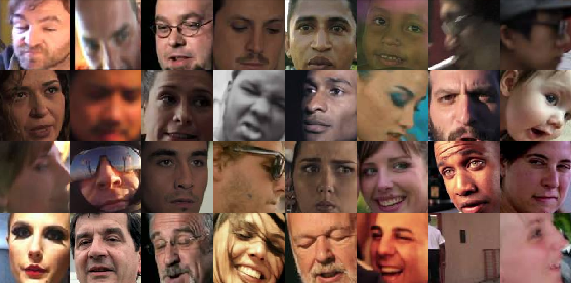
\includegraphics[width=0.98\linewidth]{img/random_sample_faces.png}
    \caption{A random selection of faces extracted from the dataset. In the bottom right corner we can see a false positive from extraction.}
    \label{fig:random_selection_faces}
\end{figure}

\section{Face similarity based on the deep features}

First of all, we were interested if the features from pretrained network contain interesting information, that could help in the search for a specific face. We used ... \todo[inline]{Add dlib more information}. This network produces a feature vector of length 128 as face representation. The authors' state, that the recommended threshold for euclidean distance for two feature vectors to be accepted as one is 0.6.

We investigated the results based on the euclidean distance and we show a result for a given face to find the closest (i.e., most similar) faces in the dataset. The sample can be seen in the figure \ref{fig:closest_faces}.


\begin{figure}
    \centering
      \begin{subfigure}[b]{\textwidth}
        \centering
        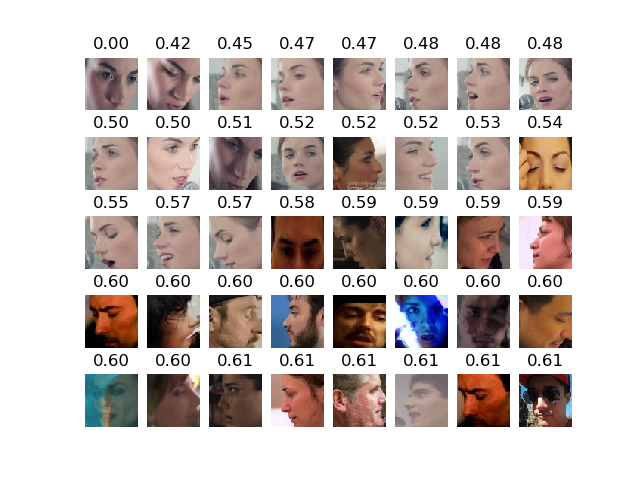
\includegraphics[width=\linewidth]{img/closest_faces_to_woman.png}
        \caption{}
        \label{fig:my_label}
    \end{subfigure}
    
    \hfill

      \begin{subfigure}[b]{\textwidth}
        \centering
        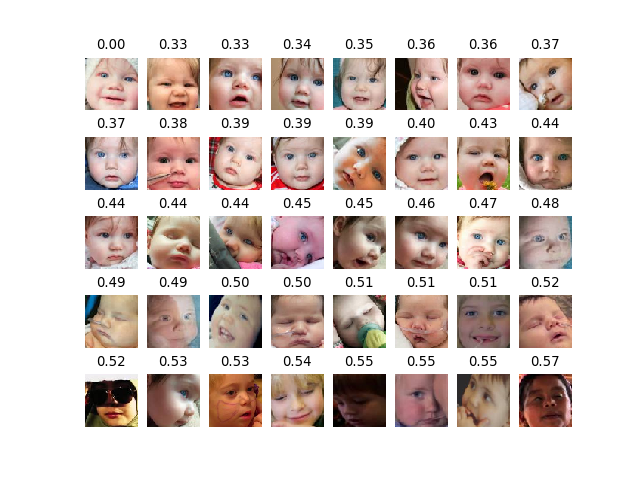
\includegraphics[width=\linewidth]{img/kid_closest_faces.png}
        \caption{}
        \label{fig:my_label}
    \end{subfigure}
    
    \caption{Examples of the retrieved closest faces to the query face (top left) based on euclidean distance. Above images is the distance from the query.}
    \label{fig:closest_faces}
\end{figure}




\section{Building a search structure}

After examinating the features and their potential we created a hierarchical structure to give a possibility to examine more faces than the user can see at screen at once.


Our solution consists of the following steps, which are further described.
\begin{itemize}
    \item Find faces
    \item Compute face encoding
    \item Train self-organizing map (SOM) from the features
    \item Build layered structure over the SOM
\end{itemize}

\subsubsection*{Find Faces}
We use pretrained CNN face detector, which is available in Dlib from custom pretrained modell….


\subsubsection*{Compute face encodings}


\subsubsection*{Train self-organizing map from the features}
Train self-organizing map from the features
// popisat preco a co su self organizing maps



\subsubsection*{Build layered structure over the SOM}

In order to project the dataset to user we need add a new layer of options - nabigation. We have seen ... success with SOM 

By creating self-organizing map we layed down a grid lattice to include all available faces. This means that the size of the map corresponds to the size of the dataset. In our case, when we work with more than TODO faces, it is unbereable to present the user with all the faces at once.

We implement tree structure sampling. Each layer contains only a subset of faces available in the next layer. This representants are chosen as every k-th image from the next layer. In other words, our final model consists of n grid lattices. Ln-1 is the bottom layer containing the full SOM. Li for i e {0,...n-2} holds: Lixy = Li+1, x*k, y*k.
